\chapter{Inter-Procedural Analysis}

Inter-procedural Analysis is required to obtain more precise results as it is very common that programs can have multiple function calls. It is essential to consider the effect of function call on the data flow value entering the node. Inter-procedural analysis takes into account call return , parameter passing , local variables of the function, return values and recursion into account. Major issue to be dealt while handling inter-procedural analysis is to deal with calling contexts. Handling concurrency also needs to be supported , which would be discussed in the next chapter. \\


\section{Context Sensitivity}
A context sensitive analysis is an inter-procedural analysis which analyses callee procedure for each context whereas context insensitive analysis performs analysis irrespective of calling context. Context insensitive analysis over-approximates inter procedural control flow which results in imprecision because it takes into account invalid control paths. Each function is analyzed once with single abstract context. Whereas context sensitive analysis is more precise as
it considers the valid inter procedural control flow. \\

Java is an object oriented language supporting features like encapsulation and inheritance. Thus data access is indirect through method calls for each class. So context sensitivity plays a very important role for Object Oriented languages.
     
\section{Call Graph}

Call Graph is graph with nodes and edges in which nodes represent procedures and there is edge from $a$ to $b$ if some call-site at $a$ calls procedure
$b$. Hence this is a static data structure that represents the run-time calling relationships among procedures in program. Soot provides a Spark engine which generates the call graph. VASCO on the other hand returns a much precise call graph, which is generated using liveness based inter-procedural pointer analysis. A thing to note here is that construction of call graph requires inter-procedural analysis and inter-procedural analysis on the other hand requires call graph. An approach to breaking this dependency is to initially approximate the call-graph and in every iteration perform inter-procedural analysis and improve the precision of the call graph.\cite{vasco} \\

Call multi-graph is a directed graph which represents calling relationships between procedures in a program where nodes represent procedures and edges procedure call. A cycle in the call multi-graph denotes recursion. Super graph is another representation in which callsites are connected to the callee procedure entry node and and the exit node of the callee is connected to return node in the caller procedure. \\     

\begin{figure}[here]
	\begin{center}
		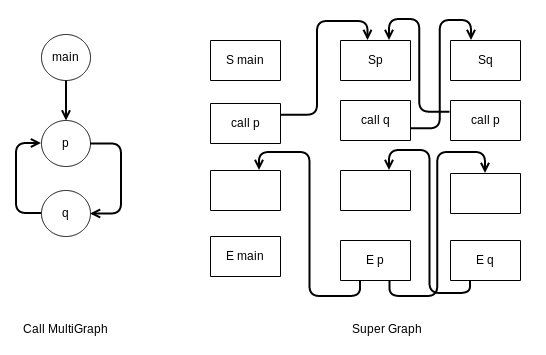
\includegraphics[scale=0.5]{Figures/callgraph.png}
	\end{center}
	\caption{Example of call multi-graph and super-graph}
	\label{fig:call graph}
\end{figure}

Data flow analysis uses static representation of programs to compute summary information along paths. For ensuring safety, all the valid paths must be covered. A valid path is the path which represents legal control flow. Ensuring precision is subject to merging data flow values at shared program points without including invalid paths. For ensuring efficiency, only those valid paths that yield information that affects the summary information should be covered.

\section{Approaches to Inter-procedural Analysis}

In this section approaches to perform inter-procedural analysis is discussed. A very simple approach is to perform procedure in-lining where every procedure call is replaced by the procedure body. This would however only be applicable when target of the call is known and call is not made by pointers or is virtual. However this is not good way to handle recursion as the code size can increase in an unbounded manner. \\

\subsection{Functional approach}

In the functional approach, summary flow functions are computed for each function. The summary flow functions are used as the flow functions for the procedure call. The summary flow function of a given procedure is influenced by the summary flow functions of the callees of $r$ and not by the callers of $r$. Also in the presence of loops or recursion, iterative computation will be needed till fixed point is achieved. Termination is only guaranteed if, lattice is finite.

\subsection{Call Strings Approach}

This is a general flow and context sensitive method. In this approach the call history is stored for information to be propagated back to the correct point. Call string at a program point is the sequence of unfinished calls reaching that point starting from the main procedure call. The data flow equations are changed to incorporate the merging of the data flow values only if the contexts(call strings) are the same. At a call node $c_i$ , $c_i$ is appended to the call-string value at that point. Similarly at a return node the last call site ci is removed. And other data flow values are blocked. For non-recursive programs number of call strings are finite. For recursive programs, number of call strings can be infinite. However, the problem is decidable for finite lattices.

There is an approach of value based termination of call-strings. This method deals with creating equivalence classes. If two call-strings have same data flow values at the start node of the procedure, then they will produce the same data flow values at the return node of the procedure call. Such call strings are grouped into equivalence classes.

An very simple example of call strings method is shown below.\cite{mtpreport}
\begin{verbatim}
public static void main ()
{
	B x;
	// Callsites are appended to the current call string before making call f and g are pointers to nodes in a linked list.
	C1 : x = after(f); 
	C2 : x = after(g);
}
B after(B a) // c1 [a = f] c2 [a = g]
{
	return a.next;
	// C1 [return f.next] C2 [return g.next]
}
// c1 [ object return would have its next pointed to f] 
// c2 [ object returned would have its next field pointed to h]

\end{verbatim}


\subsection{Value Context Method}

In this method, a combination of tabulation (functional approach) and value based termination (call strings) approach is adopted. The call-stings are partitioned based on the data flow value at the call site. And then analysis of the procedure can then be performed once for each partition. It also combines the two views of contexts: data flow values at call site are stored as value contexts and call strings as calling contexts. Distinct data flow values are maintained for each context of a procedure.\cite{vasco} \\

A value context is defined by a particular data flow value reaching a procedure. It is used to enumerate and store the summary flow function of the procedure in terms of input and output pairs. In order to compute these pairs, data flow analysis is performed within the procedure for each context(input data flow value). The out value of each context is  initialized with the top element. This approach also maintains a context transition table which allows flow of information along inter-procedurally valid paths. Transitions are recorded in the form (($X$,$c$) , $Y$) where $X$
represents calling context, $c$ represents call site and $Y$ represents callee context. Hence when analysis of callee procedure completes where to return is
identified by context transition table. Therefore propagation to valid path is guaranteed. \\

When a new call to a procedure is encountered, the context table pairs are consulted to decide if the procedure needs to be analyzed again. If it was already analysed once for the input value, output can be directly processed else a new context is created and the procedure is analysed for
this new context.

\section{Example of value context method}

\begin{figure}[here]
	\begin{center}
		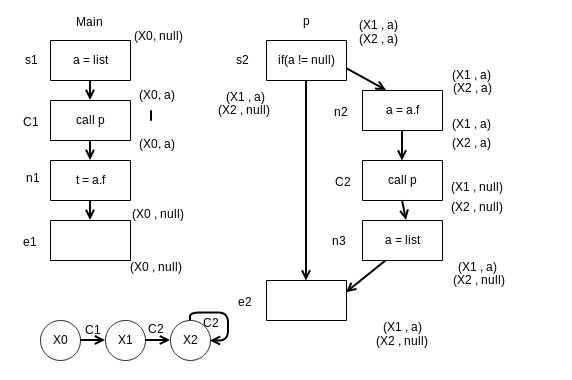
\includegraphics[scale=0.5]{Figures/interproc_example.png}
	\end{center}
	\caption{Example of value-context based IP analysis}
	\label{fig:extreme}
\end{figure}

This is an example of an inter-procedural heap liveness analysis. We wish to find out if a is live before and after the statement $C_1$ The procedure p is recursive and gets called with two different contexts $X_1$ and $X_2$ as shown in the context transition diagram as well. \\ 

The analysis starts with the intial context $X_0$ at statement e1 in main with the value null . The in value of $n_1$ is becomes $a$ as \emph{a.f} is being set to $t$ in the statement. On the next node $C_1$, we have a function call to $p$. So a new value context $X_1$ is created with input $a$ and value $null$ and the transition from X0 to X1 is noted. Now in $X_1$ context, node $n_3$ is processed followed by $c_2$, which creates another value context $X_2$ for procedure $p$ with input $null$ with value $null$. The transition $X_1$ to $X_2$ is also recorded in the context transition table. \\

In the context $X_2$, node $c_2$ is evaluated. Since there is already a context for input value $null$ we take its out value to be $null$ (the top value of the lattice). Thus, the in values of $C_2$ and $n_2$ are set to $null$ and $a$ respectively. Since $s_2$ does not kill the access path $a$, the output value of context $X_2$ is set to $a$. \\

The callers of $X_2$ are $X_1$ and $X_2$ itself. Both these contexts are now added to the work-list for processing. The only change for context $X_2$ is in the call statement $c_2$ whose in value is now set to $a$. On evaluating context $X_1$, we similarly get its output value to be $a$. After this step, the statement $C_1$ in context $X_0$ gets the in value assigned to be $a$, which gets killed in $s_1$.  \\

%X3,c2 is picked up for processing and this time the correct exit value of X2 i.e u+v- is used and so the out value of X3,c2 becomes a-b+c-. However the values do not change for its successor. Thus no more nodes of X3 need to be expanded. The process continues with X1,c2. It's out value comes out to be a+b-c- as the exit value of X2 is u+v-. X1,n3 is then picked up. The sign of c is found out to be negative and this propagates to the end of the procedure. The exit values of X1 becomes a+b-c-. And now X0,c1 is added to the work list for processing and thus q is found out to be negative. \\
%
Value based contexts are used as a cache table for distinct call sites apart from terminating analysis of recursive procedures. 


